\documentclass[12pt]{article}

\usepackage{graphicx}


\usepackage{color}
\usepackage{listings}

\usepackage[T1]{fontenc}
\usepackage[scaled]{beramono}



\usepackage{color}
\definecolor{deepblue}{rgb}{0,0,0.5}
\definecolor{deepred}{rgb}{0.6,0,0}
\definecolor{deepgreen}{rgb}{0,0.5,0}

\newcommand\pythonstyle{\lstset{
language=Python,
basicstyle=\ttfamily,
otherkeywords={self},             % Add keywords here
keywordstyle=\color{deepblue},
emph={MyClass,__init__},          % Custom highlighting
emphstyle=\color{deepred},    % Custom highlighting style
stringstyle=\color{deepgreen},
frame=tb,                         % Any extra options here
showstringspaces=false            % 
}}

\lstnewenvironment{python}[1][]
{
\pythonstyle
\lstset{#1}
}
{}


\begin{document}

\begin{titlepage}
\title{Comparison of Online Store Prices} %CHANGE!!!!!!!!
\author{Alex Kofke}
\date{STAT 312}
\maketitle
\end{titlepage}



\section{Overview}
The purpose of this experiment is to compare the average prices of a specific category of two large online stores. I chose to collect and analyze data on the ``Shoes'' section of two
online sports equipment stores, Dick's Sporting Goods and Eastbay. My goal was to collect unbiased random samples from these populations and interpret the data to determine
if there is likely an average difference in prices between the two stores in this category. I used tools in the programming language \texttt{Python} to gather data directly from the websites,
and the statistical analysis language \texttt{R} to perform computations on the samples.

Given samples from these stores, I want to learn if a difference in the sample means likely represents a difference in the population means of this category. In other words, the
null hypothesis would be that the averages are the same and the alternative, which I would like to be a stronger conclusion, is that there is a difference. For the independent samples
test, $H_0: \mu_0 = \mu_1$ and $H_1: \mu_0 \neq \mu_1$. For the paired samples test, $H_0: \mu_D = 0$, and $H_1: \mu_D \neq 0$.

\subsection{Store Selection}
Originally, I had planned to compare the Dick's online store against Amazon, and to include a much larger number of categories in the population. However, I eventually decided that
a different store and a more specific category would better suit the project. There would be many more problems attempting to extract data from the Amazon website. Amazon has a much
more open-ended collection for even a single category, and due to third-party sellers an item could have multiple prices which could not be easily extracted from the web page alone.
Additionally, Amazon has their own interface that paying partners can use to access price data, so they try to ensure that obtaining data directly from their web pages is largely 
impractical.

Eastbay, on the other hand, is a store much more similar to Dick's. It offers much of the same products and categories and is similar in scale. The way its web site is set up makes data
collection very feasible as well, so it makes sense to compare these two stores instead.

I have chosen the Shoes category over more general ``athletic apparel'' because it is large, yet does not contain too many strata. It also offers a decent range of prices to make the
experiment meaningful as well as having enough products in common to be able to conduct paired-samples testing.

\section{Data Collection}
The data collection process was a very interesting part of this study. I thought the best way to collect unbiased data was to simply extract the price data for the whole populations
 directly from the websites and then construct random samples from these data. Since there were thousands of products for each site in just this shoes category, it would be nearly impossible to go through and collect the data by hand. Therefore, I had to write programs to extract all the data I needed from the websites. This process is sometimes known as
 ``web scraping'' and there are a number of tools to help go about it efficiently. I wrote all my programs in Python, which is a language that is very friendly towards scripting of this type.
 
 Ideally, a website could have an API or Application Programming Interface, which is essentially a way to ``ask nicely'' for the data you need. However, in these instances I had to actually
 process the web pages themselves to obtain the data. This amounts to having the program ``look at'' the webpage and grab the correct prices. This is broken up into two steps
 for each website: download all of the relevant \texttt{html} files, and parse each file to find all of the product prices and save them. Python offers two libraries that help with these steps,
 \texttt{requests} and \texttt{BeautifulSoup}. The first retrieves a given web-page, and the second searches through the ``soup'' of the html file to find what you need. My strategy for gathering the price data involved getting pages with grids of product previews, each with the product name and price. 
 
 Going through and parsing a number of the pages allowed me to collect the entire populations of data for this category into two csv files. The Dick's file had a total of $2112$ entries
 and the Eastbay file had $3507$. I could then treat these data sets as the actual populations and extract random independent and paired samples. 
 
  \emph{Note: I have not attached the actual source code for my scripts since they are not currently very readable but I can provide them if needed}

 
 \subsection{Paired Data Collection}
 Finding the paired-data population to obtain samples from was probably one of the more challenging tasks. The two populations contained plenty of products in common, but the exact product titles used on the websites and therefore in the data were usually slightly different. A human could easy tell they were the same, but there was no way to match products manually
 and a simple match of text in the opposite data set would not work. So, I had to use a python library for ``fuzzy'' string matching. The fuzzy matcher computed a similarity ratio based on a 
 number of heuristics and if the ratio was high enough it would be reported as a match. Through this process I produced a set of $479$ pairs. Through trial and error I found that I had to set the threshold quite high in order to avoid a large number of false positives. The resulting paired data set therefore might not contain every equivalent product, and could still have a few false positives still.
 
 \subsection{Obtaining Random Samples}
 Fortunately, obtaining a random sample from data is very easy in python as well. I can simply give a sample size and the original population and it will produce a new set that is a simple
 random sample, without replacement. Then all I have to do is export this new sample to csv and import it with \texttt{R} to perform analysis. This library was designed specifically for computing random
 samples from a population so I am confident that the sampling is unbiased. The population is large enough that non-replacement should not affect probability of being chosen with reasonable sample sizes.

\section{Data Analysis}
\subsection{Independent Samples}
I produced an independent random sample of size $100$ from both stores and imported it to R. A box plot (Figure 2) of both samples seems to indicate that they are quite similar. The averages
look to be very close, and neither is drastically more spread than the other. The Dick's plot does indicate an outlier, and Eastbay has slightly less variability. 

Next, we will look at the normal probability plots of these samples to help determine eligibility for a t-test. The produced graph (Figure 3) show that there is some deviation from normality,
especially for the Dick's sample. However, the majority of the points lie along the lines. Since the t-test only requires approximate normality, we can run an independent samples
t-test.

Running the t-test in R produces the following results (Figure 1):

\begin{figure*}[h]
\begin{verbatim}
Welch Two Sample t-test


data:  dsg_sample$price and eb_sample$price
t = -0.0555, df = 187.368, p-value = 0.9558
alternative hypothesis: true difference in means is not equal to 0
95 percent confidence interval:
 -10.99997  10.39797
sample estimates:
mean of x mean of y 
   83.509    83.810 
\end{verbatim}
\caption{Independent Samples t-test Results}
\end{figure*}

The mean of the Dick's sample is $83.5$ and the mean of the Eastbay sample is $83.8$. The $95\%$ confidence interval for the true difference in means being zero is from $-10.99$ to
$10.39$. With the p-value being $0.955$, there is absolutely no evidence that the difference in means is statistically significant, and we cannot reject the null hypothesis.

Say that we wanted to be able to detect an average difference of $5$ dollars between the two stores. This doesn't seem like much but it's not insignificant compared to most of the
prices and in such a close competition it could make a difference. We can compute the sample size needed to detect this practically meaningful difference. First, we find the pooled
standard deviation, which turns out to be $38.35$. Next, R can calculate the required sample size with a $0.05$ significance level and power of $0.8$:

\begin{verbatim}
     Two-sample t test power calculation 

              n = 924.4433
          delta = 5
             sd = 38.35
      sig.level = 0.05
          power = 0.8
    alternative = two.sided

NOTE: n is number in *each* group
\end{verbatim}

Repeating the same calculation for a difference of one dollar gives a sample size of $n=23089$, which is much larger than either of the populations. A difference of one dollar does not
seem very significant, but it is still larger than the difference of the computed sample means. This suggests that it is unlikely we can detect even a small difference in means at a large sample size.

\begin{figure*}[h]
\centering
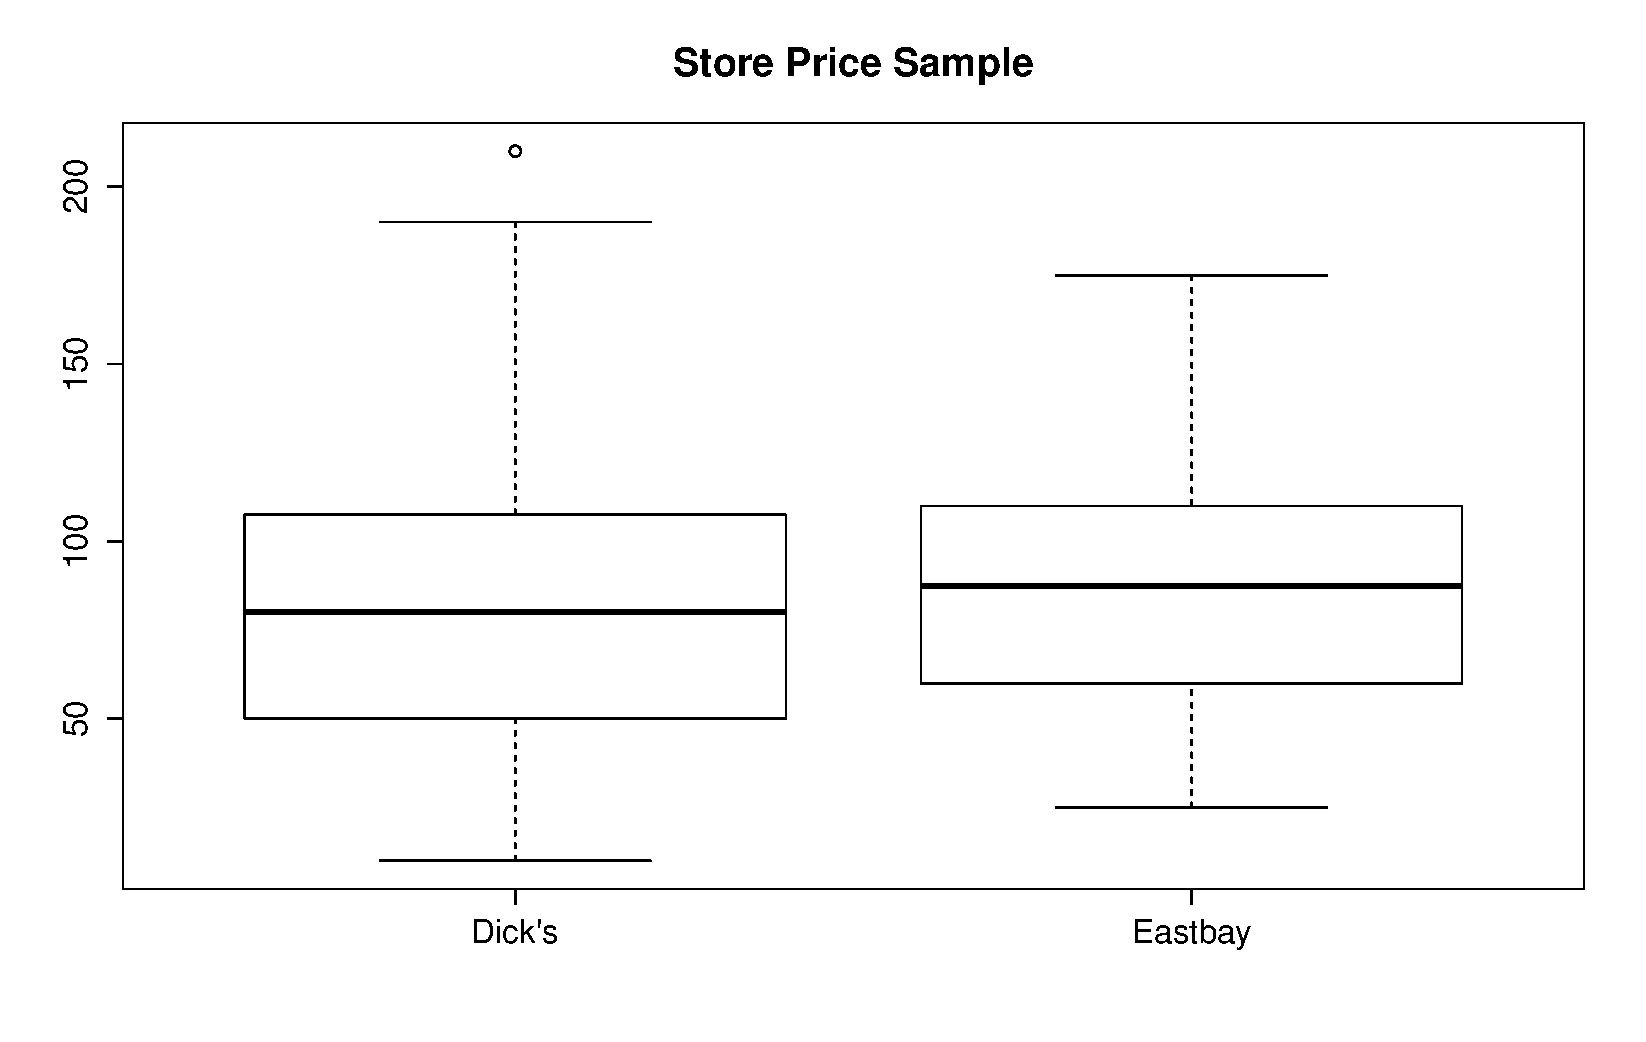
\includegraphics[width=1.0\textwidth]{samples_boxplot}
\caption{Box Plots of Samples with $n=100$}
\end{figure*}

\begin{figure*}[h]
\centering
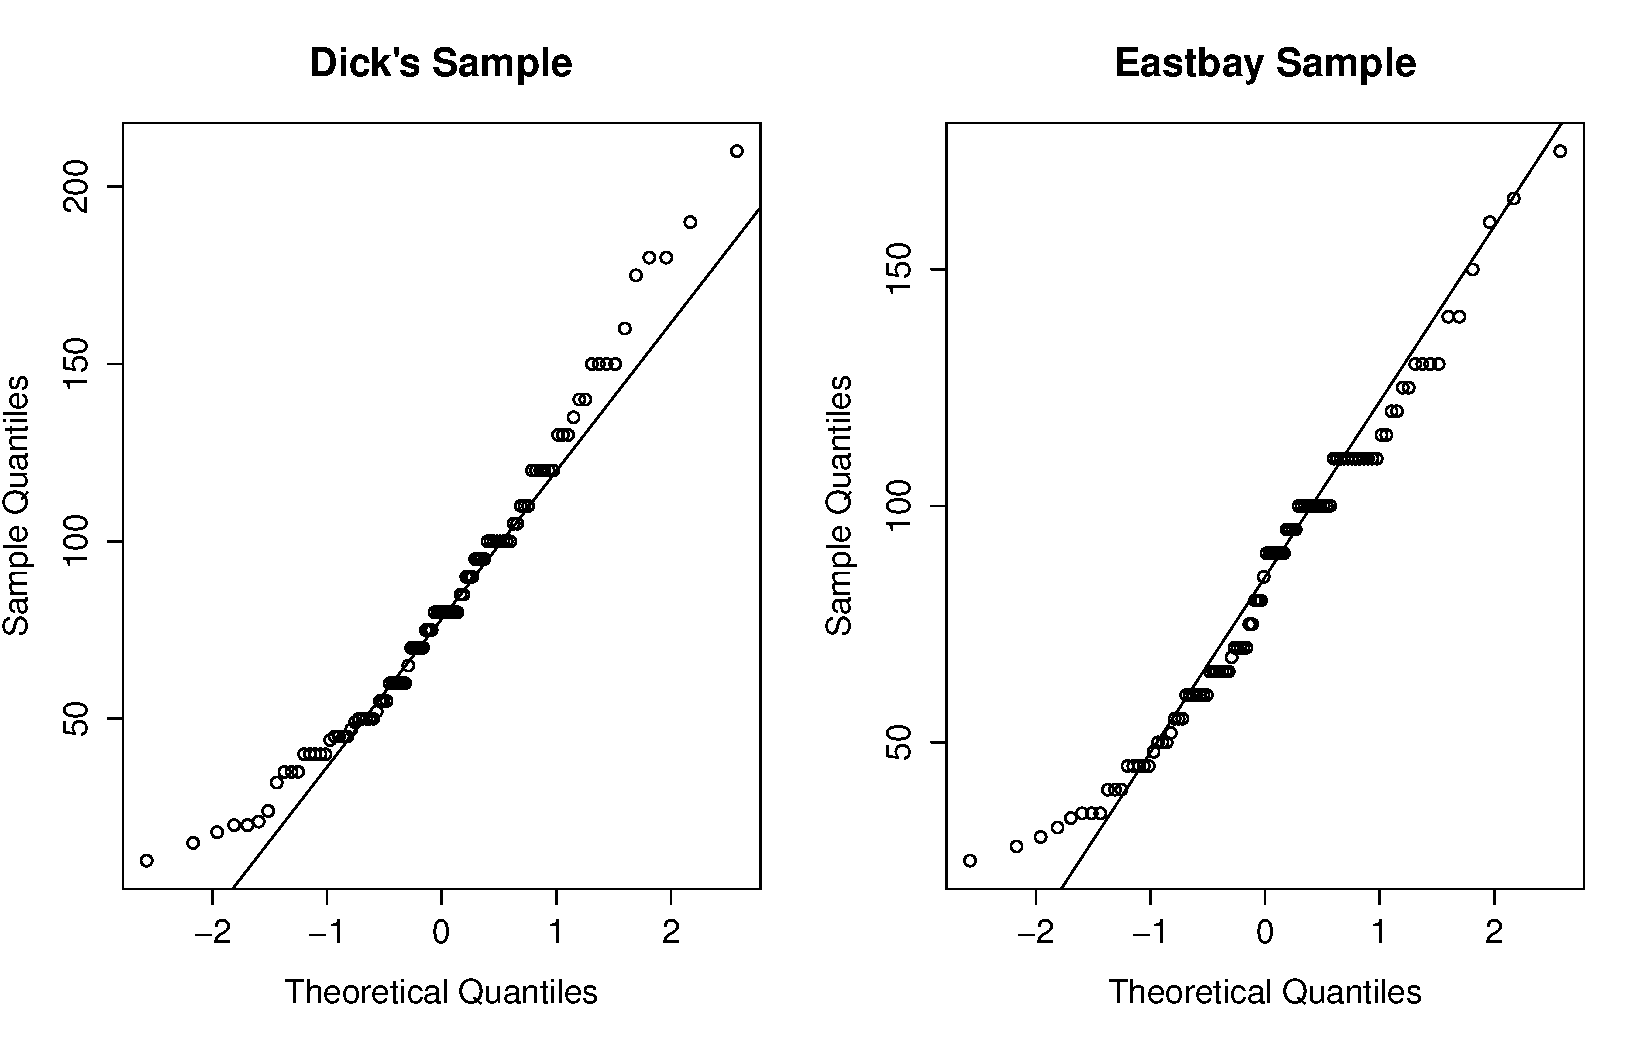
\includegraphics[width=1.0\textwidth]{samples_qq}
\caption{Normal Probability Plots of Samples with $n=100$}
\end{figure*}

\clearpage
\subsection{Paired Samples}
The data pool of paired samples is much smaller, so I chose a sample size of $50$. The null hypothesis for this test is that the mean difference of paired samples is $0$, $H_0: \mu_D = 0$, and the alternative is that there is an average difference between prices of identical products, $H_1: \mu_D \neq 0$. Plotting the differences of paired samples gives the graphs shown in Figure 4.

\begin{figure*}[h]
\centering
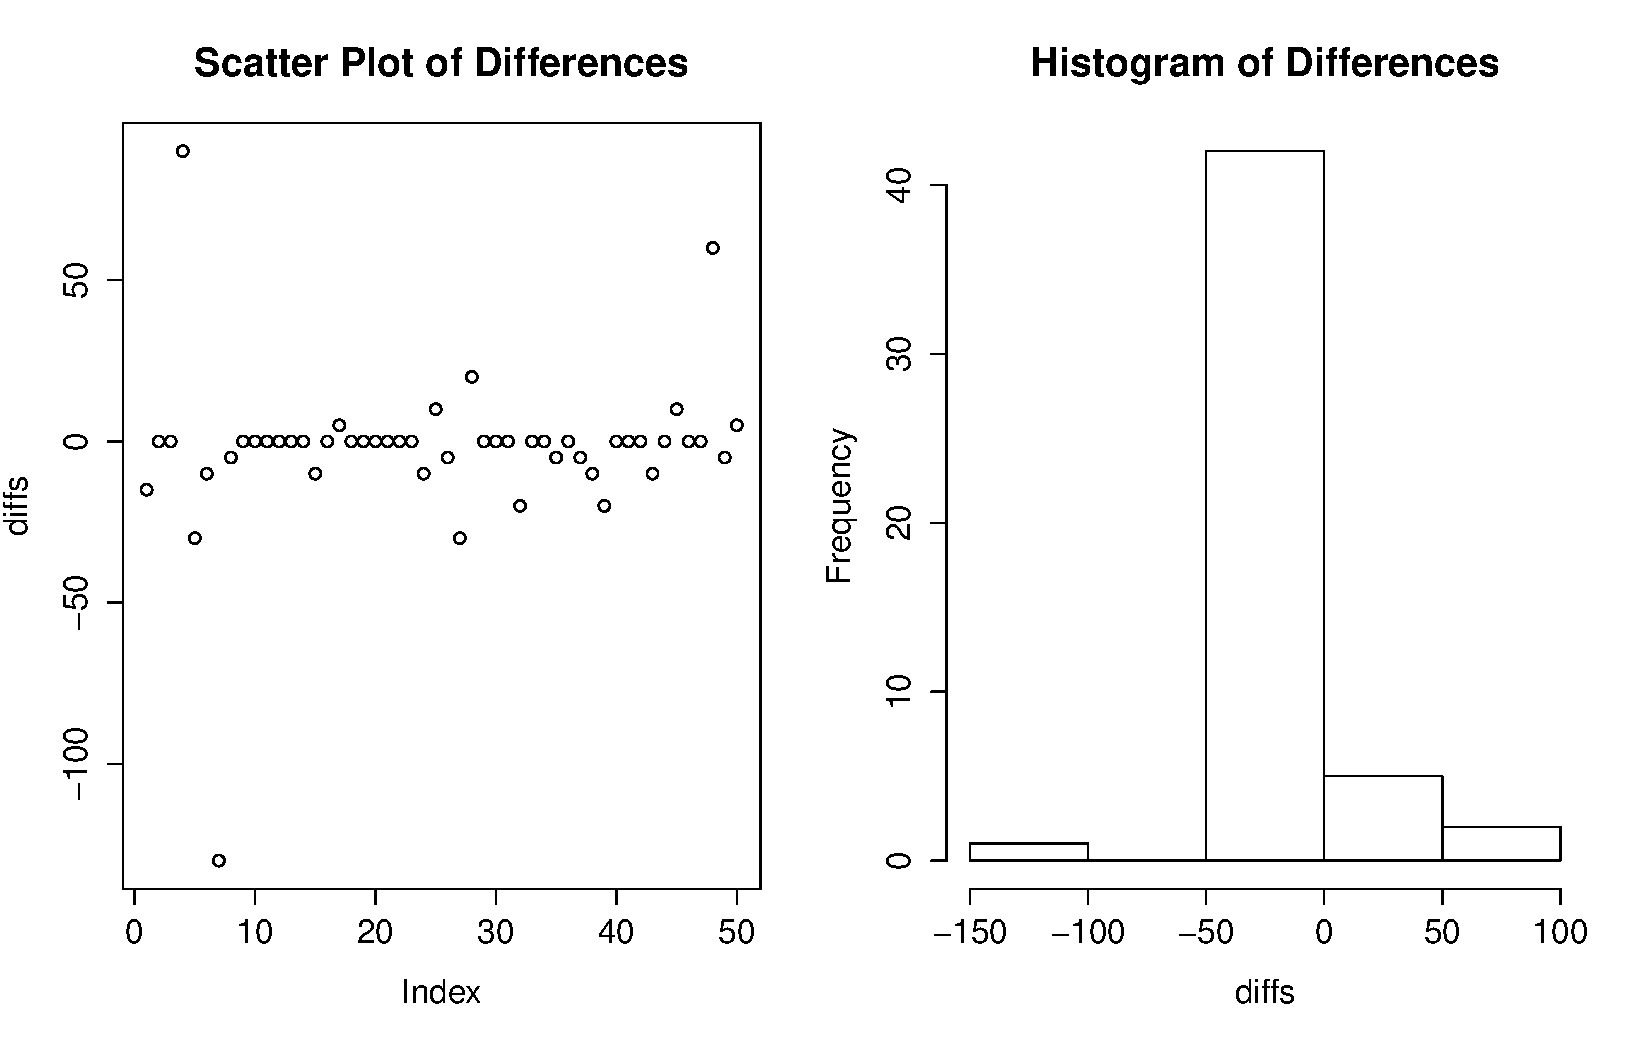
\includegraphics[width=1.0\textwidth]{diffs}
\caption{Plots of Paired Sample Differences with $n=50$}
\end{figure*}

These graphs show quite clearly that the differences are mostly zero. Some of the extreme outliers are most likely due to errors with the fuzzy matching, but the differences closer to $0$
are probably actual differences between the store prices. The normal probability plot of the differences (Figure 5) shows the same strange outliers but otherwise the points lie very close to the line.

\begin{figure*}[h]
\centering
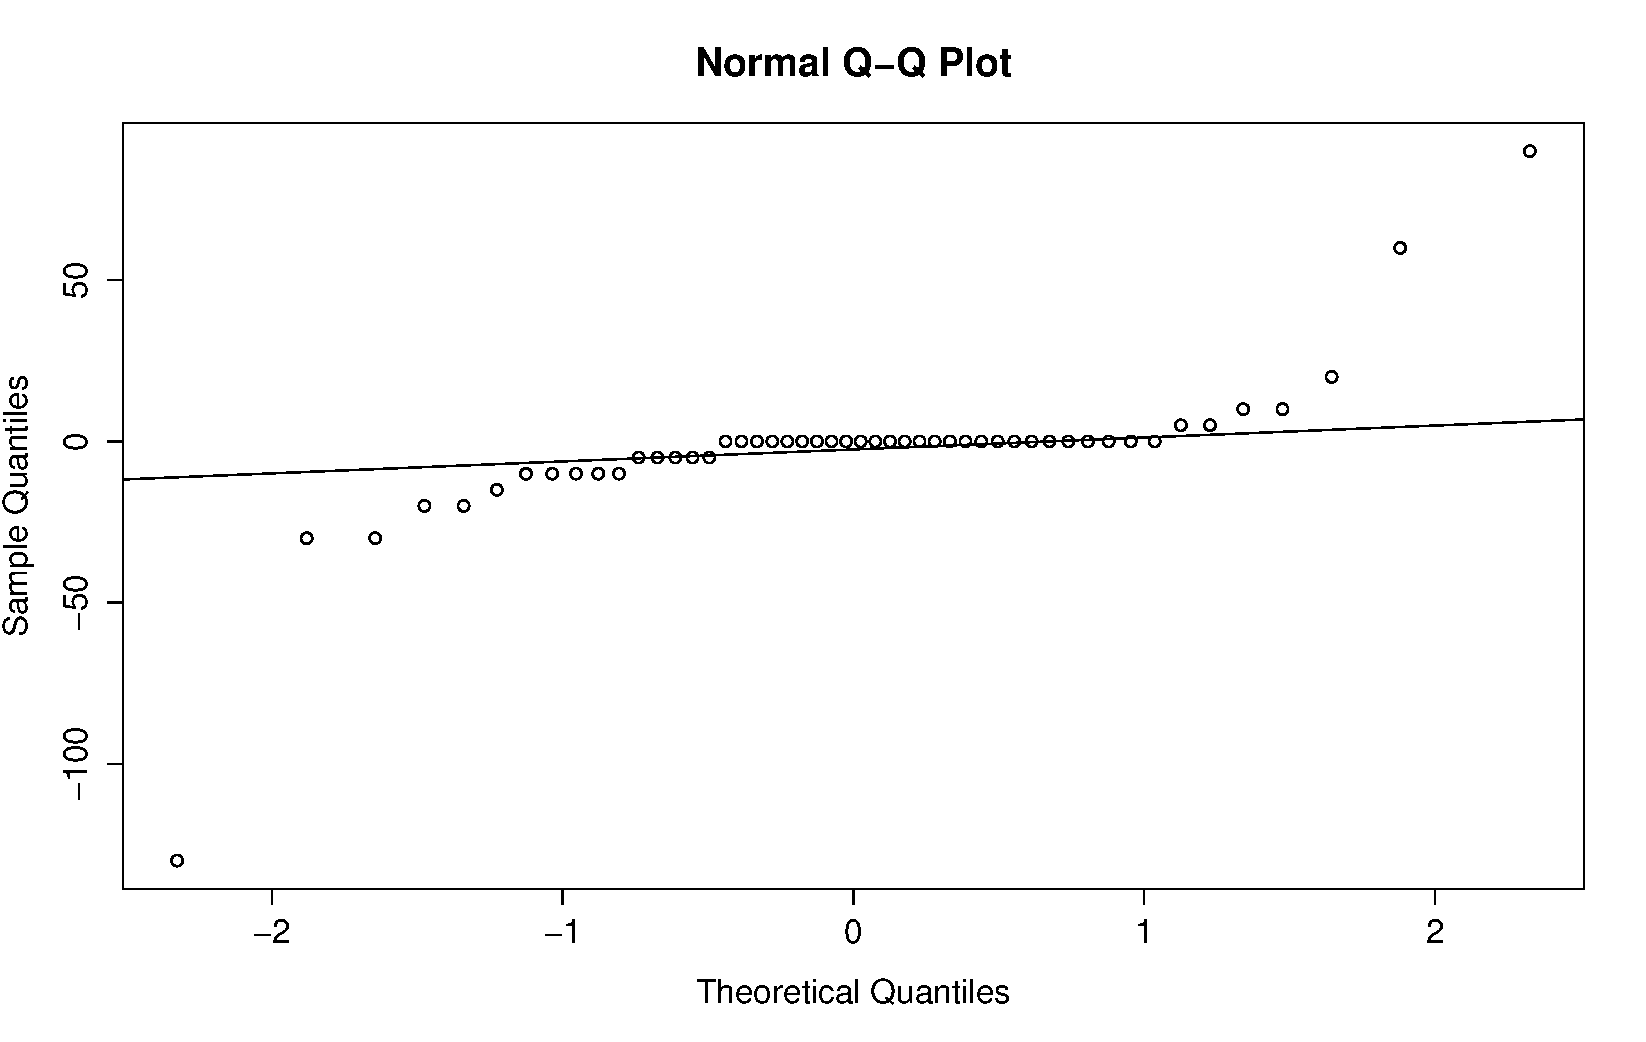
\includegraphics[width=1.0\textwidth]{diffs_qq}
\caption{Normal Probability Plot of Paired Sample Differences with $n=50$}
\end{figure*}

The results of the paired-samples t-test from R are given below in Figure 6. The $95\%$ CI for the true average difference of paired products being $0$ is from $-9.71$ to $4.90$, while the mean of the differences is $-2.4$. This gives a p-value of $0.51$ and we can easily say that there is nothing to suggest that the same products have different prices across the two stores.

To detect another price difference of $5$ dollars between pairs, the same sample size test can be run for paired t-tests. The sample size needed for this, $210$, is quite significant
compared to the size of the available population.
\begin{verbatim}
     Paired t test power calculation 

              n = 209.616
          delta = 5
             sd = 25.72
      sig.level = 0.05
          power = 0.8
    alternative = two.sided

NOTE: n is number of *pairs*, sd is std.dev. of *differences* within pairs
\end{verbatim}

 

\begin{figure*}[h]
\begin{verbatim}
Paired t-test

data:  paired$dsgPrice and paired$ebPrice
t = -0.6602, df = 49, p-value = 0.5122
alternative hypothesis: true difference in means is not equal to 0
95 percent confidence interval:
 -9.710711  4.908311
sample estimates:
mean of the differences 
                -2.4012 
\end{verbatim}
\caption{Paired-Samples t-test with $n=50$}
\end{figure*}

\section{Conclusion}
After collecting a significant amount of data for prices in the shoes categories of online stores Dick's Sporting Goods and Eastbay, all tests seem to show that there is no practical 
difference in pricing between the two stores. An independent samples test showed that neither store's average price for shoes is higher than the other, and a paired samples test showed that when comparing the same product across the stores, there is on average no difference in price. These results do make sense in the real world, as the stores are in competition and
generally would not let the other get an edge in pricing. Additionally, identical products from the same manufacturer purchased for retail would not allow for much variation in selling price.
Still, these results are not readily apparent to any browser of the sites, and so this can definitely be a useful conclusion. 
 

\end{document}
